\documentclass[12pt]{article}
\usepackage[a4paper]{geometry}
\usepackage[myheadings]{fullpage}
\usepackage{fancyhdr}
\usepackage{lastpage}
\usepackage{graphicx, wrapfig, subcaption, setspace, booktabs}
\usepackage[T1]{fontenc}
\usepackage[font=small, labelfont=bf]{caption}
\usepackage{fourier}
\usepackage[protrusion=true, expansion=true]{microtype}
\usepackage[spanish]{babel}
\usepackage{sectsty}
\usepackage{url, lipsum}
\usepackage{hyperref}
\usepackage{fancyhdr,lipsum}


\hypersetup{
    colorlinks=true, %set true if you want colored links
    linktoc=all,     %set to all if you want both sections and subsections linked
    linkcolor=blue,  %choose some color if you want links to stand out
}
\urlstyle{same}


\newcommand{\HRule}[1]{\rule{\linewidth}{#1}}
\onehalfspacing

\setcounter{secnumdepth}{2}
\setcounter{tocdepth}{5}

%-------------------------------------------------------------------------------
% HEADER & FOOTER
%-------------------------------------------------------------------------------
\pagestyle{fancy}
\fancyhf{}
\setlength\headheight{15pt}
\fancyhead[L]{SSII}
\fancyhead[R]{\uppercase{Instalación de Sistemas Operativos}}
\fancyfoot[R]{Page \thepage\ of \pageref{LastPage}}

%-------------------------------------------------------------------------------
% TITLE PAGE
%-------------------------------------------------------------------------------

\begin{document}

\title{ \normalsize \textsc{SISTEMAS INFORMÁTICOS\\
I.E.S FRANCISCO DE LOS RÍOS}
		\\ [2.0cm]
		\HRule{0.5pt} \\
		\LARGE \textbf{\uppercase{Instalación de Sistemas Operativos}}
    \HRule{0.5pt} \\
    \HRule{2pt} \\ [0.5cm]
    %\normalsize  \vspace*{10\baselineskip}
    \LARGE \textbf{\uppercase{MANJARO}}
    \HRule{2pt} \\ [0.5cm]
    \normalsize  \vspace*{2\baselineskip}
    }

\author{
        Trabajo realizado por: \\
		Antonio Muñoz Cubero
	    \normalsize  \vspace*{4\baselineskip}
		}
\date{\textbf{01 de Febrero de 2021}}
\newpage
\maketitle
\newpage

%-------------------------------------------------------------------------------
% Table of Content
\tableofcontents
\newpage
%-------------------------------------------------------------------------------

%-------------------------------------------------------------------------------
% Section title formatting
\sectionfont{\scshape}
%-------------------------------------------------------------------------------






%-------------------------------------------------------------------------------
% BODY
%-------------------------------------------------------------------------------


    \section*{Introducción}
      En el transcurso de esta práctica seguiremos los pasos adecuados para que la Instalación del sistema 
      operativo, en este caso \textbf{Manjaro} se realice de manera satisfactoria. También hemos de cumplir 
      una serie de criterios para la correcta realización de la misma, que son los siguientes.
      \begin{itemize}
        \item Instalación del sistema. Elige (justifica tu elección y asigna los recursos a la máquina virtual 
        según los requisitos de la distribución elegida) e instala una distribución de Linux en máquina virtual 
        (el nombre del sistema será el nombre de usuario del alumno/a de moodle). (captura de pantalla al asignar 
        el nombre de la máquina).
        \item Particionamiento del sistema. Muestra el particionamiento del sistema que has realizado durante la 
        instalación (Captura si aparece en el asistente).
        \item Actualización del sistema. Utiliza la herramienta gráfica para comprobar si el sistema está actualizado 
        (Captura de pantalla).
      \end{itemize}
      

      \newpage

      \section{Creacion de la máquina virtual}
      El primer paso de esta práctica es la creación y configuración de una máquina virtual adecuada para la instalación 
      del sistema operativo que vayamos a utilizar, en nuestro caso usaremos \textbf{Manjaro}. Para ello, abrimos 
      nuestro programa de virtualización y le damos a añadir una nueva máquina virtual y nos desplegará el siguiente menú
      en el caso que usemos \textit{virtual box}
      \begin{figure}[h]
        \centering
        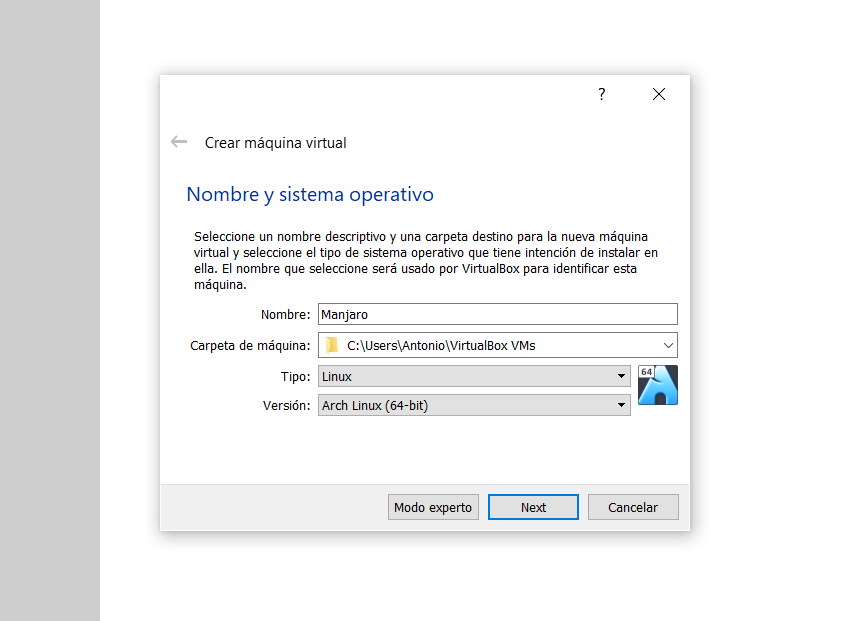
\includegraphics[scale = 0.5]{img/manjaro_install_1.png}
        \caption{Creacion de la máquina virtual.}
        \label{Manjaro1}
      \end{figure}

      La configuración de la máquina virtual está hecha acorde a los requisitos mínimos del sistema, que previamente hemos 
      buscado. Tras esto, solo hemos de confirar la máquina virtual siguiendo dichos requisitos.

      \begin{figure}[h]
        \centering
        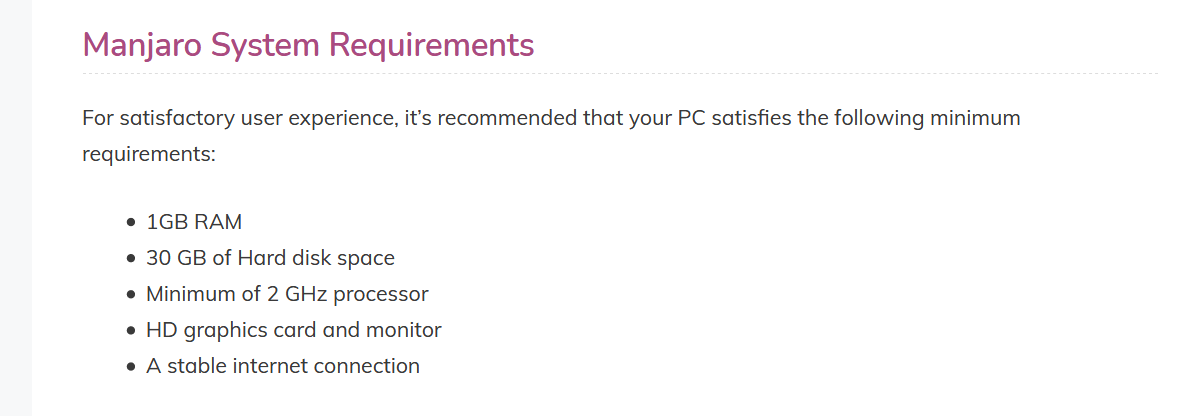
\includegraphics[scale = 0.4]{img/requisitos.png}
        \caption{Requisitos mínimos Manjaro.}
        \label{requisitos}
      \end{figure}

      \newpage

      Ahora simplemente, rellenamos los campos que nos piden con los parámetros adecuados para el correcto 
      funcionamiento del sistema.

      \begin{figure}[h]
        \centering
        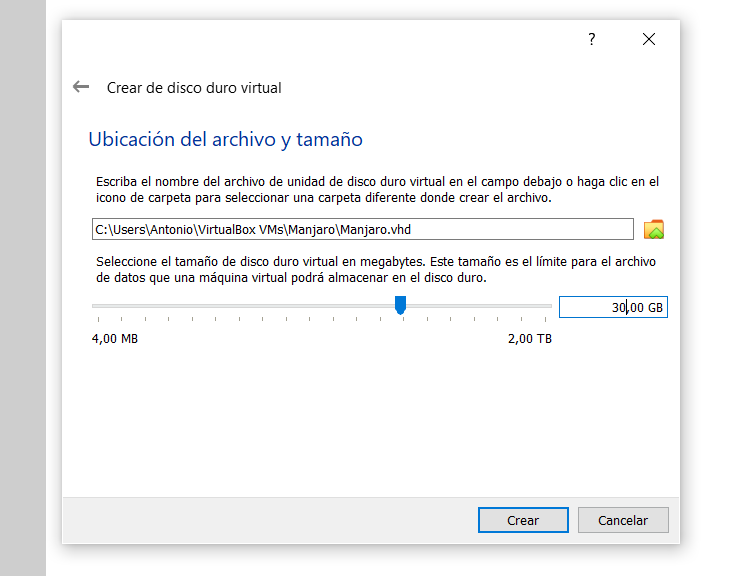
\includegraphics[scale = 0.5]{img/manjaro_install_3.png}
        \caption{Creacion de la máquina virtual.}
        \label{Manjaro2}
      \end{figure}

      \begin{figure}[h]
        \centering
        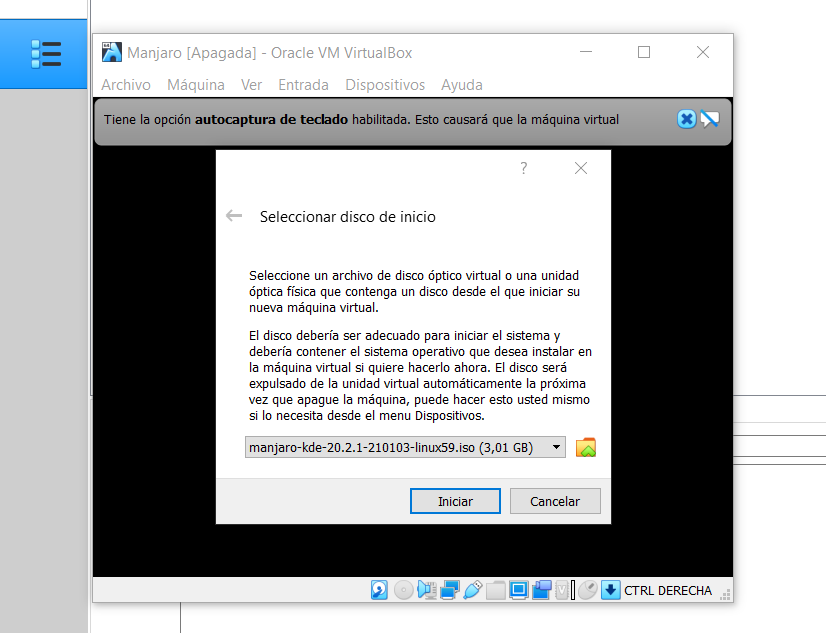
\includegraphics[scale = 0.5]{img/manjaro_install_4.png}
        \caption{Creacion de la máquina virtual.}
        \label{Manjaro3}
      \end{figure}
    
      Una vez seguidos estos pasos, nuestra máquina virtual estará creada y lista para su funcionamiento. Ahora 
      nos queda montar la imagen y proceder a la instalación. Para montar la imagen, arrancamos la máquina y seleccionamos 
      la ubicación de la iso.

      \newpage

      \section{Instalación de Manjaro}
        Lo primero que vemos al iniciar la imagen de Manjaro es un asistente que nos permite cambiar una serie de parámetros 
        para la instalación y nos pregunta si queremos usar drivers libres o propietarios.\\
        Configuramos el idioma, teclado y hora acorde a nuestro lugar de residencia o preferencia.\\
        Tras ello, yo continuaré con drivers de codigo libre.

        \begin{figure}[h]
          \centering
          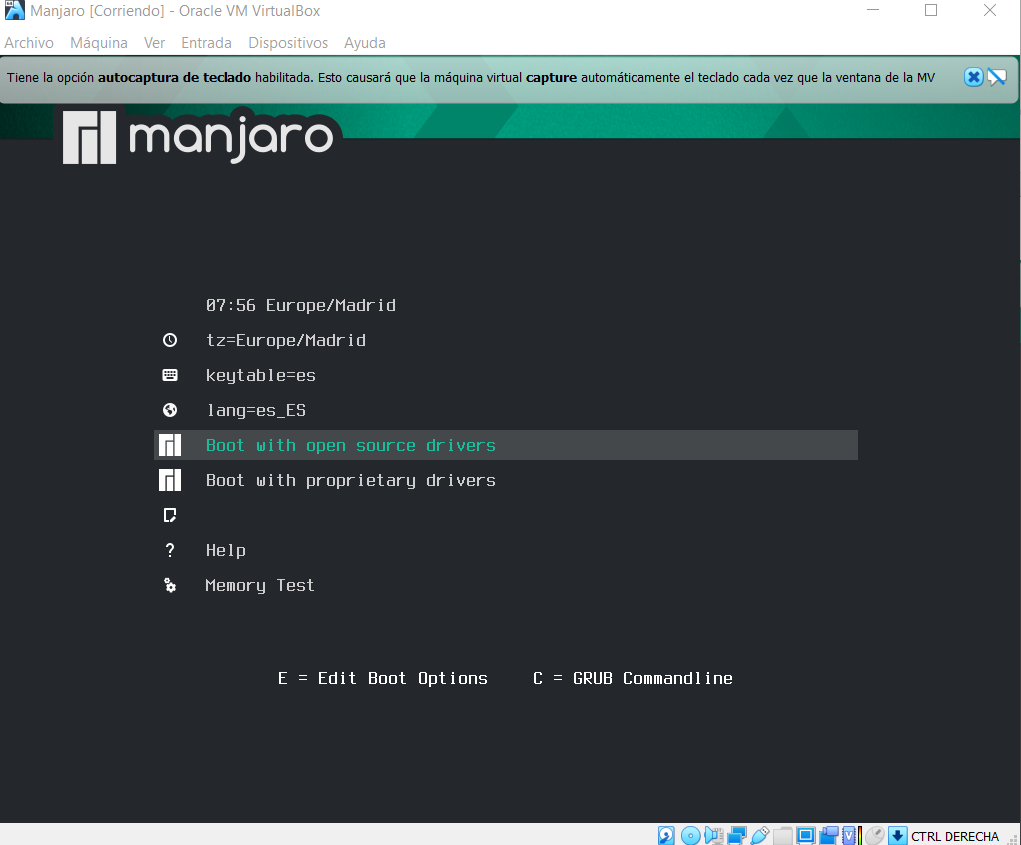
\includegraphics[scale = 0.4]{img/manjaro_install_8.png}
          \caption{Asistente Manjaro.}
          \label{Manjaro4}
        \end{figure}

        En el sigiuente paso, selecionamos la opcion de instalar y el idioma Español.

        \begin{figure}[h]
          \centering
          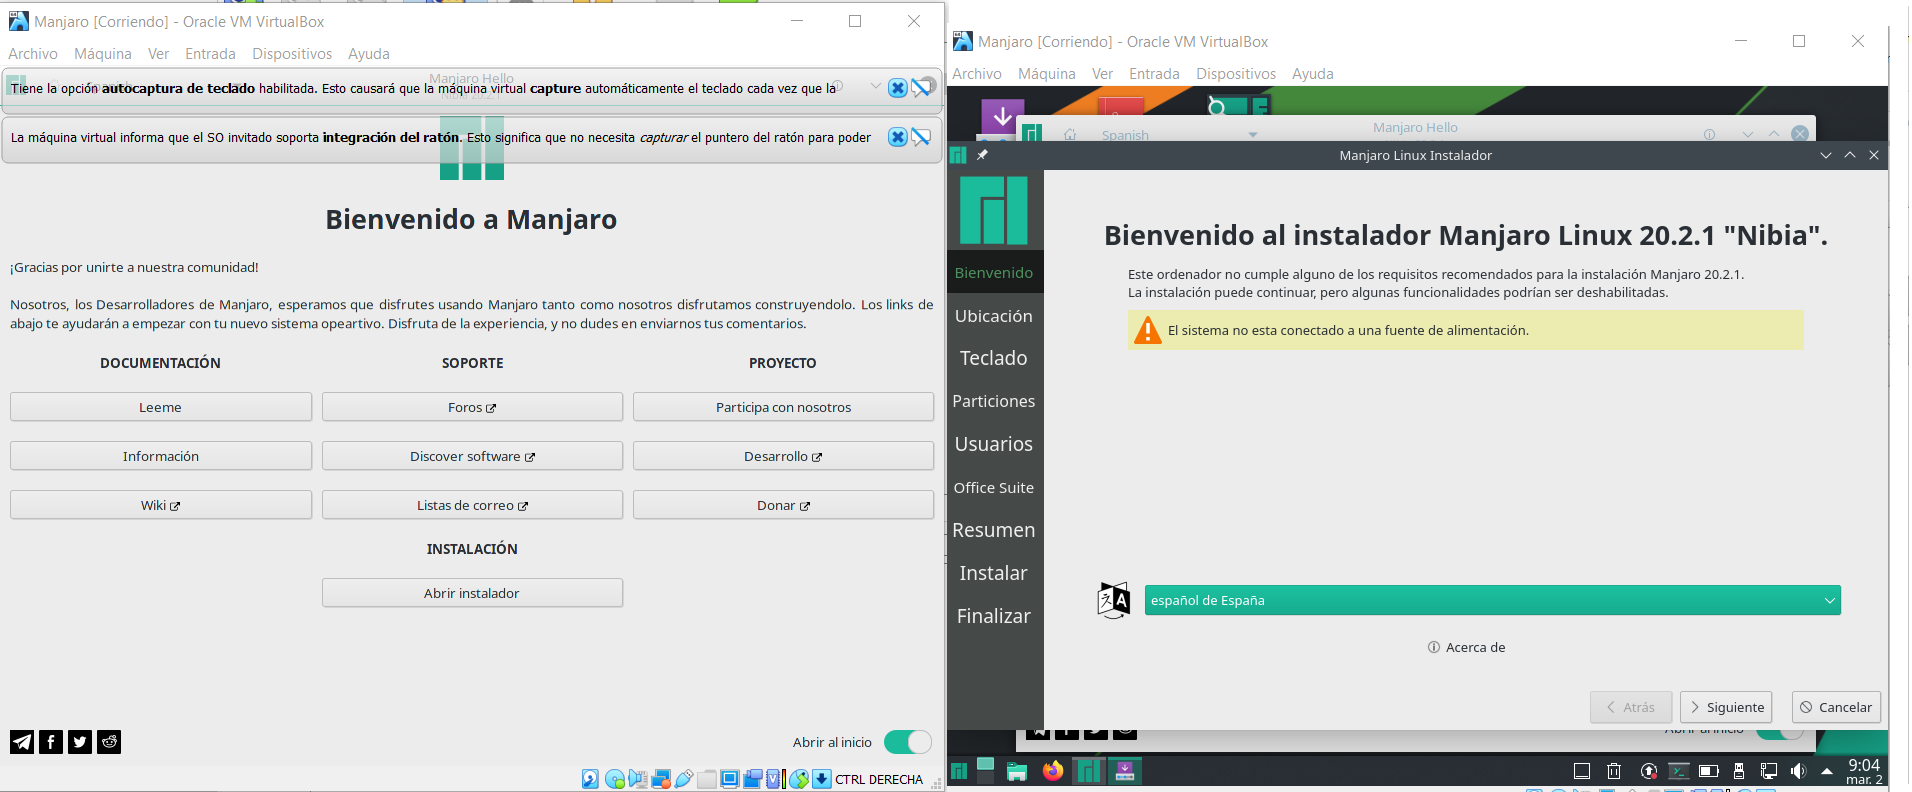
\includegraphics[scale = 0.35]{img/manjaro_install_10.png}
          \caption{Instalador de Manjaro.}
          \label{Manjaro5}
        \end{figure}

        \newpage

        Acto seguido seleccionamos la zona horaria y la distribución de teclado que usamos.

        \begin{figure}[h]
          \centering
          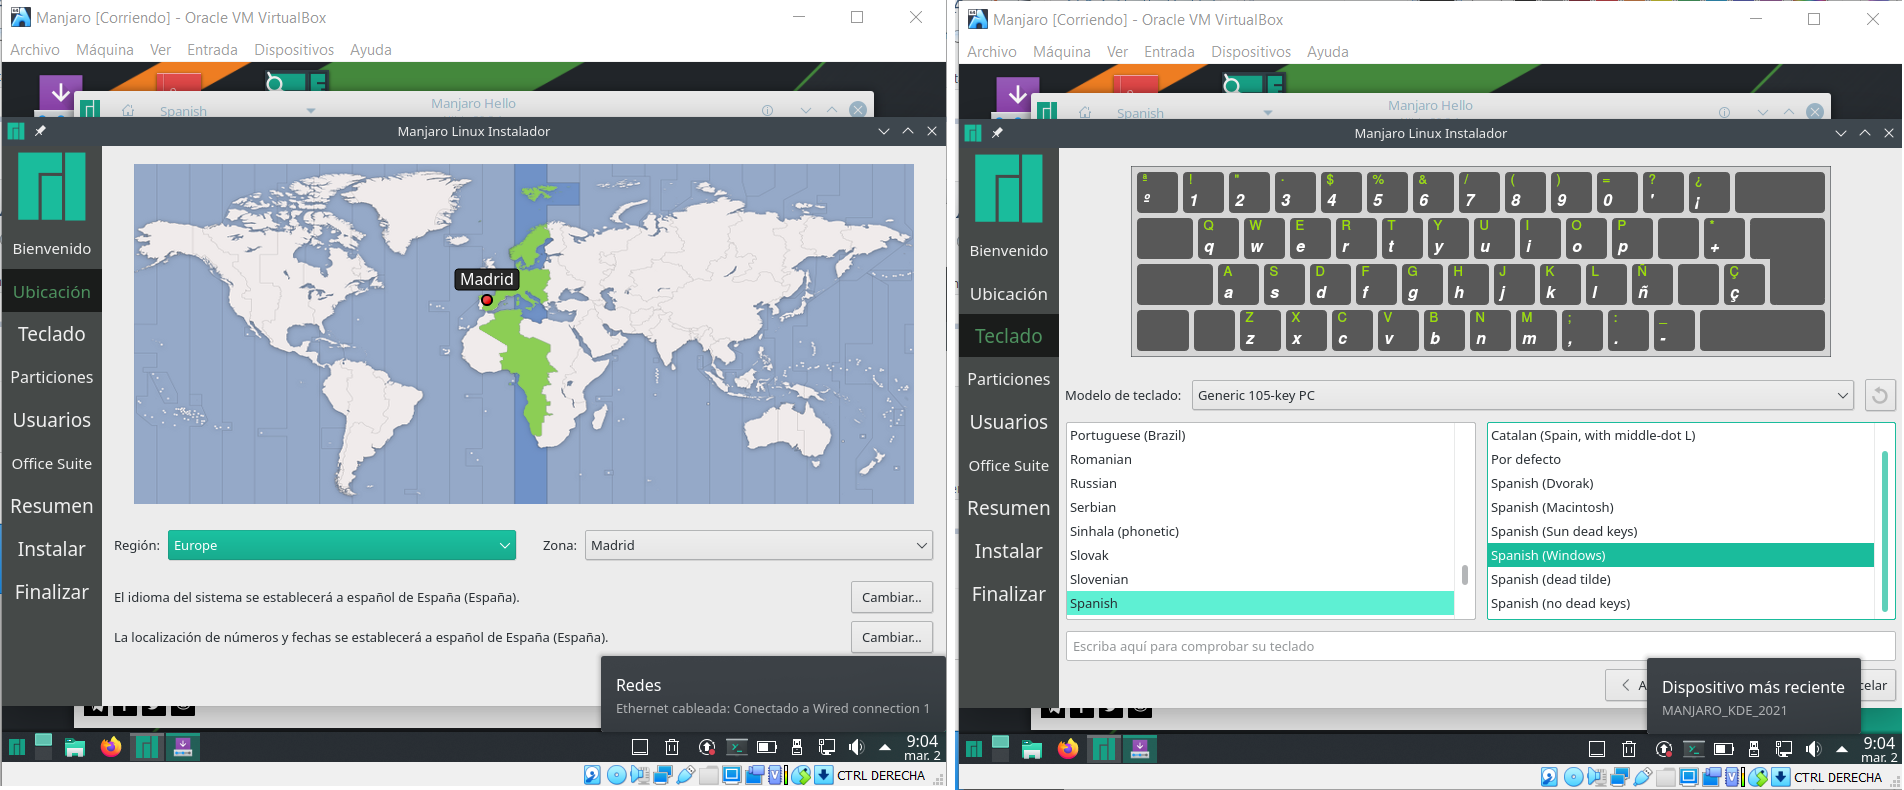
\includegraphics[scale = 0.35]{img/manjaro_install_11.png}
          \caption{Instalador de Manjaro.}
          \label{Manjaro6}
        \end{figure}

        Acto seguido nos preguntará si queremos hacer una partición manual o automática, elegiremos la 
        primera opción, y en la siguiente ventana rellenaremos los campos del usuario y contraseña para 
        seguir con la instalacion del sistema operativo.

        \begin{figure}[h]
          \centering
          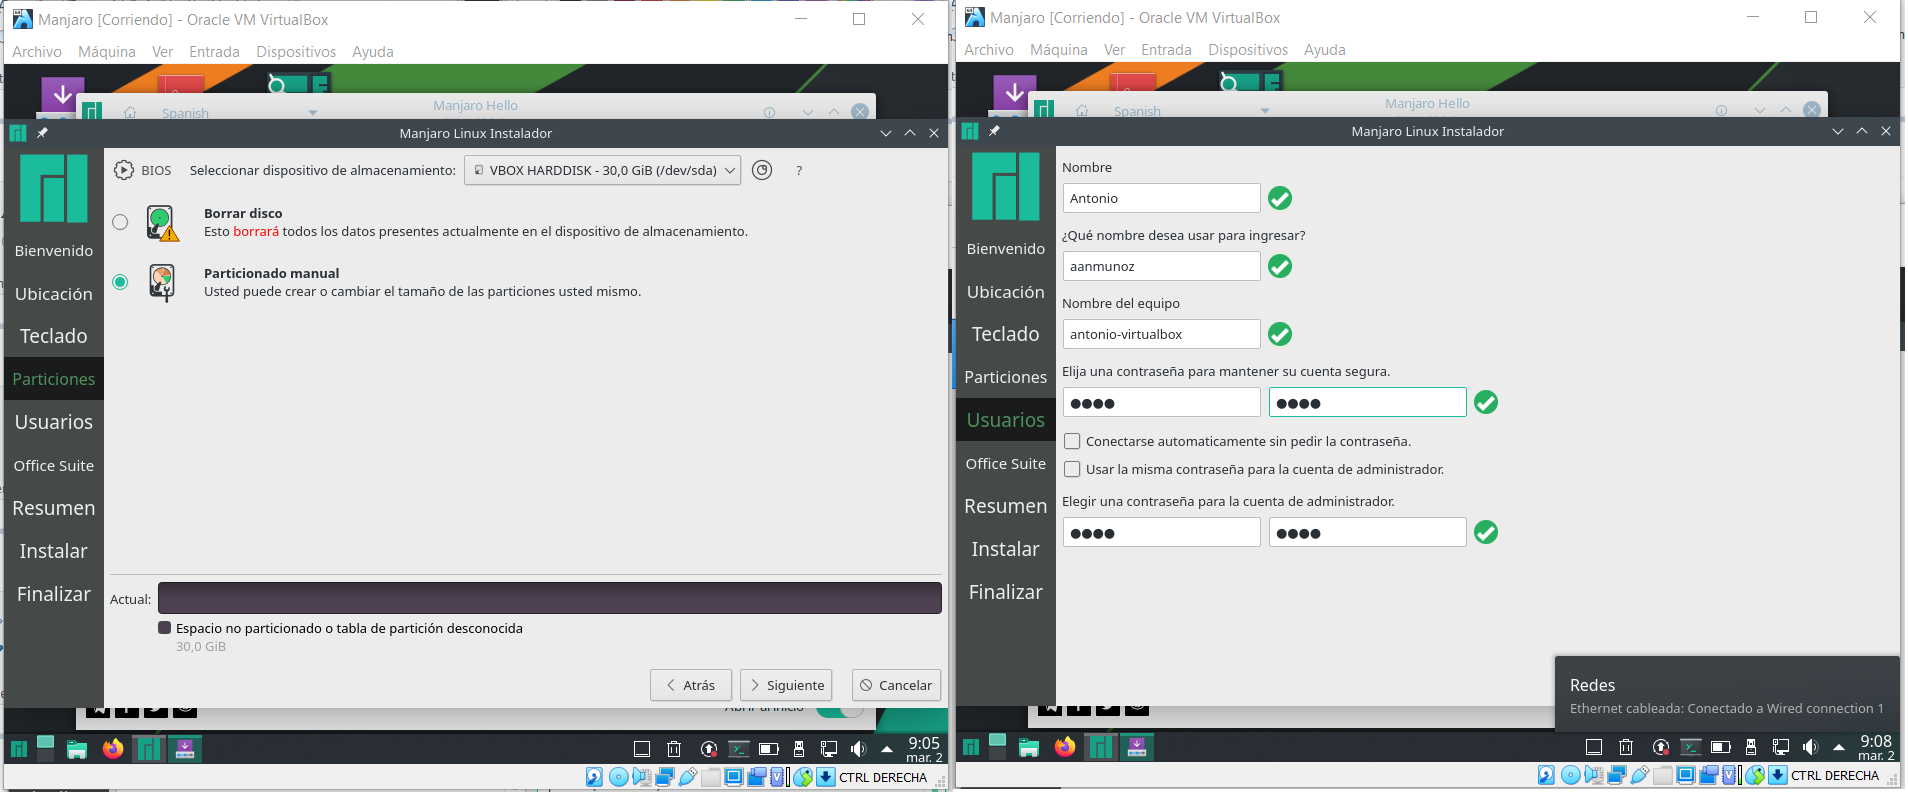
\includegraphics[scale = 0.35]{img/manjaro_install_13.png}
          \caption{Instalador de Manjaro.}
          \label{Manjaro7}
        \end{figure}

        Despues de esto, nos mostrará un resumen de lo que hemos elegido y procederá con la instalación, ahora 
        solo nos queda esperar a que el sistema se instale.

        \newpage 

        Una vez nuestro sistema está instalado para buscar las actualizaciones del sistema, solo tenemos que introducir 
        \textit{Actualizaciones} en el buscador del inicio.

        \begin{figure}[h]
          \centering
          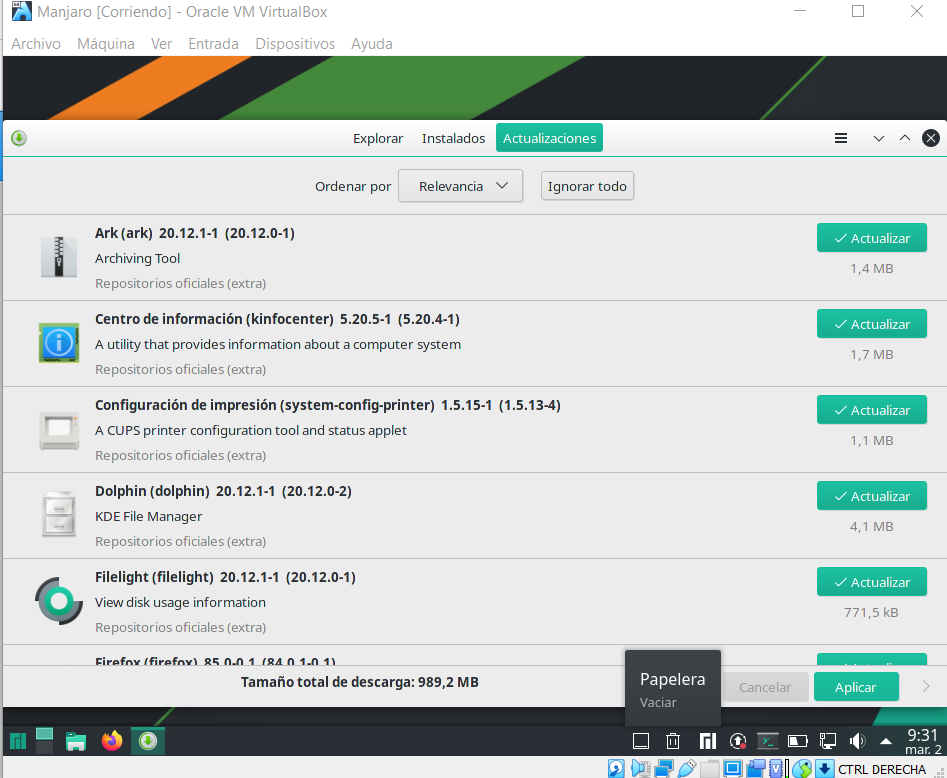
\includegraphics[scale = 0.5]{img/manjaro_install_21.png}
          \caption{Actualizaciones del sistema.}
          \label{Manjaro7}
        \end{figure}









      \newpage

      \section{IMÁGENES}
      \listoffigures
        
  \end{document}